\section{Nand to Tetris and the Hack Architecture} \label{hack-architecture}
Nand to Tetris is divided into several sections that can be worked on or skipped more or less independently of each other.
Each section describes a higher level of abstraction in the hack architecture, the computer system designed to be implemented throughout the course.
In the beginning, the students create the necessary chips and logic gates to build a full CPU, starting with only a not-and (NAND) gate.
This section is not part of this thesis, but it may become relevant in future additions to the application~\ref{future-work}.
After that, students work with the Hack assembly language~\ref{hack-assembly} and create their own assembler whose generated code targets the CPU created in the previous section.
The application created as part of this work contains an emulator that can run that assembly directly without further compilation.
This allows students to run their assembly code in the same application as their VM code from the later sections.
Next, students work closely with VM bytecode, first writing a translator from bytecode to assembly, and later writing a complete game using the high-level programming language Jack, which was designed for this course.
At the end, students create their own compiler for said high-level language.
They will also implement a standard library for it that abstracts many of the direct interactions with the platform, such as printing text to the screen.
The last two parts are relevant to this project because students can run both the VM code and their compiled assembly in the emulator.
The main focus of this project is on the game mentioned above, which is created in Project 9.
It may seem strange to develop a whole new emulator mainly to improve a single project out of twelve, but this one exercise is the ``Tetris'' referred to in the title of the course.
Although Project 9 is not the final project, for many it is the highlight of the course.
This is illustrated by the fact that nine of the twelve examples listed under the ``Cool Stuff''~\cite{n2tweb} tab on the official website are Jack programs that would qualify as Project 9 solutions.
So if the goal is to improve the overall student experience, it makes sense to focus on this part.
Nevertheless, the emulators created as part of this thesis can also improve the experience for other projects~\ref{evaluation}.
It is important to keep in mind that both the bytecode and the assembly are theoretically intended as intermediate steps for compiling Jack code into machine language, even though this project is about interpreting them directly.
The entire pipeline with many of the relevant terms that will be used throughout the thesis is shown in~\cref{fig:hack-pipeline}.

\begin{center}
  \begin{figure}[ht]
    \centering
    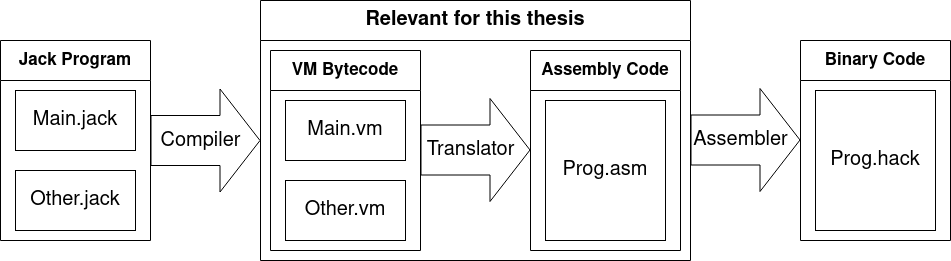
\includegraphics[width=14cm]{fig/hack-pipeline.png}
    \caption{The transformation from Jack code to machine code.}
    \label{fig:hack-pipeline}
  \end{figure}
\end{center}

% \subsection{The sections of Nand to Tetris}
% \begin{itemize}
%   \item Chips und Logic Gates (nicht Teil der Arbeit)
%   \item CPU und Assembly
%   \item Virtuelle Machine
%   \item High level Sprache und Betriebssystem (nicht Teil der Arbeit)
% \end{itemize}
%
\subsection{Hack assembly} \label{hack-assembly}
There are three different languages in the Nand to Tetris course that are relevant for this work.
The first and least complex of the three languages is assembly language.
Assembly language in this case simply means that the language has a direct mapping to machine language that the CPU can actually understand.
Each assembly instruction can be mapped to a single number that can be interpreted directly by the machine's hardware.
Assembly in modern systems is often complicated with a plethora of instructions~\cite{guide2011intel}, but hack assembly has only two.
These two instructions are used to manipulate two physical registers called A and D.
In addition, there is a third register called M, which is actually just the memory cell pointed to by the address in the A register.
This allows the assembly to work without any dedicated instructions for memory manipulation.
Every register and memory cell has a width of two bytes.
The first instruction is called the A instruction because its only purpose is to write a constant value into the A register.
In assembly code it is written as \verb+@value+, so for example \verb+@42+ would write the value 42 into the A register.
The C instruction, on the other hand, can perform a plethora of different functions.
These range from negating the value of a single register to performing a binary-or operation on two registers and jumping to another instruction if that value is greater than zero.
The destination of that jump would be determined by the value inside the A register.
C instructions consist of one or more destination registers, an equal sign, an expression, e.g.\ D-A, and a jump if necessary.
A deeper understanding of how hack-assembly works is not required to understand the following sections.
\cref{lst:hack-assembly} shows a simple assembly program, which checks if the value in memory at address 3 is equal to 5 and if so, jumps to instruction 100.

\begin{lstlisting}[
  language=HackAsm,
  caption={A simple Hack assembly program~\cite{nisan2005}.},
  label={lst:hack-assembly},
  captionpos=b]
@3
D=M   // D := RAM[3]
@5
D=D-A // D := D - 5
@100
D;JEQ // if (D == 0) goto 100
\end{lstlisting}

\subsection{Hack bytecode}
\label{hack-bytecode}
% \subsection{The operating principles of the Hack VM}
Hack bytecode is the most important language for this thesis, as it is the language interpreted by the VM emulator.
Since it has way more instructions than the assembly, it makes sense to start with an example instead of explaining each instruction in detail.
The simple C program in~\cref{lst:c-add-123} shows how one might write a loop that adds the numbers 1, 2, and 3 together.
In mathematical notation, it would be written as \(\sum_{i=1}^{3}i\).
This program may seem unremarkable at first glance, but it incorporates quite a few significant concepts of modern programming languages, such as variables, loops, conditions, and arithmetic operations.
Although the program itself is trivial, its translation into machine code and subsequent execution by the computer is not.
Since machine code is highly dependent on the target architecture, the following section is specific to the Hack platform. That being said, the concepts discussed are relevant not only for most other VM implementations, but also for machine code generated by a C or Rust compiler.
This is especially true for the stack, which is an essential concept in almost every programming language.

C is an imperative language, which means that we have to tell the computer how to calculate the result instead of just telling it what we want.
The program begins with the declaration of two variables called \(i\) and \(sum\).
The first is used to hold the number of iterations performed, while the second holds the final result, which is the sum of all \(i\) we iterated over.

\begin{lstlisting}[
  language=C,
  caption={A C program to calculate \(\sum_{i=1}^{3}i\).},
  label={lst:c-add-123},
  captionpos=b]
  int i = 1;
  int sum = 0;
  while (i <= 3) {
    sum += i;
    i++;
  }
\end{lstlisting}

To translate the program above into something that can be interpreted by the Hack VM, a stack is used.
% A stack is an abstract data structure with only two fundamental operations: Push and Pop.
% The push operation adds an element to the top of the stack, while the pop operation removes the top element.
% This means that the element that was pushed onto the stack last is removed first when a pop is performed.
% For this reason, the stack model is called last-in-first-out (LIFO)~\cite{nisan2005}.
This stack model is simple but powerful and allows a very elegant description of calculations.
For example, to perform an addition, first both operands are pushed onto the stack, then the addition instruction pops these two numbers from the stack and pushes the result of the addition onto it instead.
This is illustrated in~\cref{fig:stack-add}, where 2 is pushed on top of 1 before adding both.
% The stack is often represented as growing downward, but in the Hack architecture it actually grows upward, so this representation is more appropriate.

\begin{center}
  \begin{figure}[ht]
    \centering
    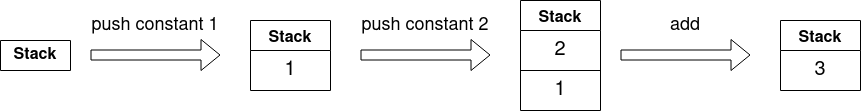
\includegraphics[width=14cm]{fig/stack-add.png}
    \caption{Adding 1 and 2 in a stack based VM.}
    \label{fig:stack-add}
  \end{figure}
\end{center}

Unlike many other architectures, push and pop in the Hack architecture can also be used to read and write arbitrary memory addresses, so no other memory-related instructions are required. For this reason, they are the only instructions in Hack that can manipulate memory outside the stack.
This is made possible by extending both instructions with a segment and an index. The segment acts as an offset that the VM adds to the index that follows it.
The address for the instruction is therefore computed as \(address=offset(segment)+index\).
It is used either as the destination where the result of a pop operation is written, or as the source location of a value to be pushed.
\cref{table:segments} in the appendix shows all eight possible segments and their purpose, but only the following two are required to understand the example in~\cref{lst:hack-bytecode}.
The local segment gets its location in RAM from the first memory cell: \(address=RAM[1]+index\).
So a \verb+pop local 3+ would perform the following operation: \(RAM[RAM[1]+3] = pop()\).
In contrast, the constant segment differs from all other segments in that it does not add anything to the index before treating the result as an address, but simply pushes the index directly onto the stack without performing a memory read.
This means that the constant segment cannot be used with the pop instruction.

With this knowledge the bytecode~\ref{lst:hack-bytecode} becomes readable.
It is important to note that the bytecode presented assumes that the segments have already been initialized and therefore will not work if executed as a standalone program.
The code starts by initializing \(i\) and \(sum\) to one and zero respectively, just like the C code~\ref{lst:c-add-123}.
Afterwards, a label is declared, which is simply a position in the bytecode that can be used as a target for goto instructions.
The loop is implemented between this label and the label on the last line and can be divided into three parts.
The first part performs the exit condition check to determine if the loop body should be executed.
To do this, it first puts the value of \(i\) on the stack and then jumps out of the loop if \(\neg(i < 4)\), which is equivalent to \(i > 3\).
If the aforementioned check was false, the loop body is executed.
This means that the actual implementation of a loop condition works the other way around than in the C example, where we enter the loop if the condition was true.
This inversion is done because the code does not perform a jump when the loop is executed.
Since most loops are run more than once, this saves a lot of jumps in the program flow.
To update \(sum\), the VM loads the current value of \(sum\) onto the stack, then the current value of \(i\), and after adding the two, the result is written back to \(sum\).
Updating \(i\) works basically the same way, but with a constant value of one instead of another local variable being added.
Then we simply jump back to the beginning of the loop, where the next check for the exit condition is performed, and continue this process until that condition is met.

\begin{lstlisting}[
  language=Hack,
  caption={A Hack VM program to calculate \(\sum_{i=1}^{3}i\).},
  label={lst:hack-bytecode},
  captionpos=b]
  // i = 1
  push constant 1
  pop local 0

  // sum = 0
  push constant 0
  pop local 1

  label LOOP_START

  // the Hack bytecode does not have an <= instruction,
  // therefore use i < 4 instead of i <= 3
  // if i >= 4 jump out of the loop
  push local 0
  push constant 4
  lt
  not
  if-goto LOOP_END

  // sum = sum + i
  push local 1
  push local 0
  add
  pop local 1

  // i = i + 1
  push local 0
  push constant 1
  add
  pop local 0

  // jump to the beginning of the loop again
  goto LOOP_START
  label LOOP_END
\end{lstlisting}

\cref{table:vm-instructions} lists most instructions in the VM bytecode.
As they all work the same way, \verb+add+ represents every instruction which pops two arguments from the stack, such as \verb+and+, \verb+lt+ (less than) or \verb+sub+.
The ``Arguments'' column here refers to arguments given in the source code, such as \verb+local+ and \verb+1+ for the instruction \verb+push local 1+.
This differs, for example, from the addition instruction, which takes its arguments from the stack.
TOS is an abbreviation for top of stack, the value which was pushed last.

\begin{table}[h]
  \begin{center}
    \centering
    \begin{tabular}{@{}lllll@{}}
      \toprule
      Name     & Purpose                                                        & Arguments \\
      \midrule
      add      & Add the two numbers on top of the stack                        & - \\
      not      & Bit-invert the value on TOS                                    & - \\
      neg      & Multiply the TOS with -1                                       & - \\
      push     & Push \(RAM[offset(segment)+index]\) onto the stack             & segment, index \\
      pop      & Pop the TOS and write it to \(RAM[offset(segment)+index]\)     & segment, index \\
      label    & Declare a label, i.e., a name referring to a line of code       & label \\
      goto     & Jump to the specified label                                    & label \\
      if-goto  & Jump to the label, which is passed as an argument if TOS != 0  & label \\
      function & Declare a new function and push \(n_{local}\) zeros to the stack & function name, \(n_{local}\) \\
      call     & Call a function with \(n_{args}\) arguments                     & function name, \(n_{args}\) \\
      return   & Return from a function                                         &         - \\
      \bottomrule
    \end{tabular}
    \caption{The Hack VM bytecode instructions.}
    \label{table:vm-instructions}
  \end{center}
\end{table}

\subsection{Hack test scripts} \label{test-scripts}
The third and last language relevant to this thesis, is the test script language.
This language is special, because students participating in the course usually do not interact with it directly, which is also why the scripts do not appear in~\cref{fig:hack-pipeline}.
Instead, Schocken and Nisan already supplied test scripts for most of the exercises in the book themselves.
These scripts are used both by students, to determine if they solved the exercise correctly, but also by the teachers grading the project submissions.
Test scripts can automatically load a program, initialize values in the emulator's memory, run the program, and compare the memory after running for a certain number of ticks with a set of expected values.
An example of such a script can be seen in~\cref{lst:hack-test-script}.
All the commands, which are specific to a single simulator, in this case the VM emulator, are highlighted in red.
The script starts by loading the program it is supposed to test, in this case \verb+MyProgram.vm+.
Loading behaves differently for each emulator, as the VM emulator is also able to load an entire directory, while the CPU emulator can only load a single file.
In order to test the functionality of a program, it is necessary to specify the memory addresses which should be compared and their respective expected values.
This is done in the next three lines.
After executing the program, the values specified in \verb+output-list+ will be written in the format dictated after the \verb+%+-Symbol into the \verb+output-file+.
In the case of~\cref{lst:hack-test-script} this means that the values at addresses \verb+256+ and \verb+300+ are written to \verb+MyProgram.out+, each with one byte of padding left and right and a length of six for the value itself.
The format here is decimal, as specified by the \verb+D+.
Before this can happen, however, the program must be executed.
For this purpose, the test script can first set any value in the emulator's memory to a constant value.
This is done with the \verb+set+ command, which is specific to each emulator, since each emulator has different requirements.
For example, the CPU emulator does not understand the meaning of \verb+sp+ (stack pointer) or \verb+local+ because these terms are specific to the VM emulator.
When everything is set up, the emulator is interpreted step by step inside the repeat statement.
In this case \verb+42+ VM ticks are executed.
The instruction to drive the emulator has a different name for each one, but behaves basically the same.
Finally, the \verb+output+ command writes all values from the \verb+output-list+ into the \verb+output-file+, which is then compared to the \verb+compare-to+ file.
These two files should be identical if the program was executed correctly.
Otherwise, an error is reported.

\begin{lstlisting}[
  language=HackScript,
  caption={A simple script to test a bytecode program (red means simulator-specific).},
  label={lst:hack-test-script},
  captionpos=b]
load MyProgram.vm,
output-file MyProgram.out,
compare-to MyProgram.cmp,
output-list RAM[256]%D1.6.1 RAM[300]%D1.6.1;

// this is the segment setup required for the bytecode example to work
set sp 256,        // sp contains the address of the top of the stack
set local 300,     // the base address of the local segment

repeat 42 {        // run for 42 ticks
  vmstep;
}

// outputs the values specified in output-list to the output-file
output;
\end{lstlisting}
